\section{Cache Optimizations}
\label{sec:cache_opt}

Our cache optimizations for DNN training are based on the sparse nature of performance-critical data (e.g., activations and errors).  Our approach improves cache performance through a compact representation of cache lines containing only zeroes (a.k.a. \emph{zero cache lines}) in the caches, which helps to avoid  the normal bandwidth and storage costs of zero cache lines. These optimizations enable efficient scaling of model size and training threads. 

Managing zero data at cache line granularity makes it possible to realize our optimizations through simple and efficient extensions of existing memory systems.  Our current design comprises of mechanisms for achieving the following: (i) compact representation of zero cache lines, (ii) a parallel cache hierary for zero cache lines, and (iii) tracking zero cache lines in the memory system.  We describe these mechanims in the rest of this section.

\subsection{Zero Cache Line Representation}
Our compact representation of zero cache lines exploits the fact that data bytes are not required to represent such lines in the caches, the address tag is sufficient for this purpose. Thus, the data bytes of a zero cache line are not tranferred in the cache hierarchy, but are rather synthesized in the processor (on a read) or in main memory (on a writeback) for use, as appropriate.  However, it is important to quickly determine whether cache hit references a zero cache line or not so that the appropriate data transfer steps can be taken.  We considered two alternatives for handling this: (i) an extra bit of metadata to provide this distinction, and (ii) a cache hierarchy for zero cache lines which is accessed in parallel with the regular cache hierarchy.  We adopt the later option in our current work. 

\begin{figure}[!t]
\centering
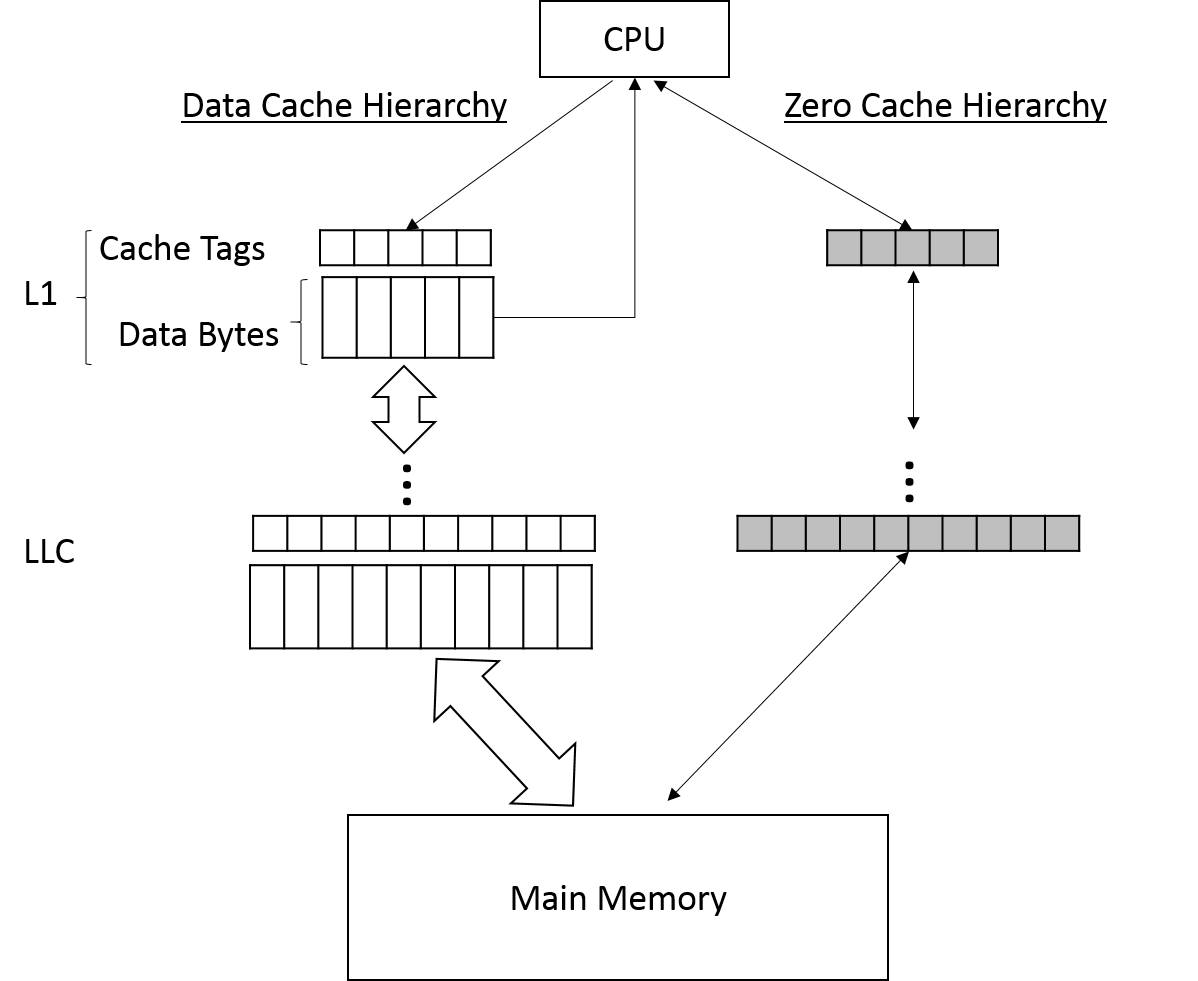
\includegraphics[width=2.4in]{Figures/zero_cache_hierarchy.png}
\caption{Memory System with Zero Cache Hierarchy.}
\label{fig:zero_cache_hierarchy}
\end{figure}

\subsection{Zero Cache Hierarchy}

Figure~\ref{fig:zero_cache_hierarchy} illustrates a memory system augmented with cache hierarchy for zero cache lines. This structure is similar to a hierarchy of conventional caches, but without the data bytes. It is designed to parallel the conventional data cache hierarchy in terms of number of levels, number of entries, ways and associativity, and inclusion/exclusion policy. It is exclusive with the data cache, since zero cache lines are not maintained in the data caches. It can be maintained across cores using the same coherence protocol.   We describe how the two cache hierarchies are accessed in parallel to satisfy data access requests from the processor. 

\subsection{Tracking Zero Cache Lines}

We track zero cache lines in the memory system, as they originate from main memory and are transferred through the zero cache hierarchy. We describe how to detect transitions of cache lines from zero to non-zero status based on processor writes, and describe a protocol for migrating cache lines between the data caches and zero caches. 

